\chapter{Testowanie}

\section{Środowisko testowe}

Aplikacja została zbudowana i testowana na komputerze stacjonarnym z systemem operacyjnym Windows 10. Specyfikacja jednostki testowej prezentuje się następująco:

\begin{itemize}
\item procesor Intel Core i5-4670K 3.40GHz
\item karta graficzna Nvidia GeForce GTX 770
\item pamięć RAM 8 GB DDR3
\item dysk twardy SSD Crucial CT120M
\end{itemize}

\section{Zestaw danych testowych}

Jako zestaw danych wejściowych, dla których testowany był algorytm układania planu zajęć, wybrany został zestaw fińskiej szkoły ponadpodstawowej. Opart on został na danych z roku 2006 szkoły West-Pori High School, gdzie wiek uczniów należy do przedziału 16-19 lat. Zestaw został wybrany z uwagi na rozmiar danych oraz duże podobieństwo siatki zajęć do polskiego gimnazjum.

Wyżej wspomniany zestaw danych zawiera jedną instancję problemu układania planu zajęć. W instancji tej występuje:

\begin{itemize}
\item 35 okien czasowych rozłożonych na 5 dni w tygodniu (maksymalnie 7 zajęć dziennie),
\item 18 dostępnych nauczycieli,
\item 13 sal, w których mogą być prowadzone zajęcia,
\item 10 grup uczniów,
\item 172 wydarzenia o łącznej długości 297 okien czasowych (wiele zajęć dwu i trzy godzinnych).
\end{itemize}

Pokrycie okien czasowych w tym planie zajęć wynosi około 85\%. Liczba ta jest stosunkiem łącznej długości wydarzeń do całkowitej liczby dostępnych okien czasowych dla wszystkich grup (35*10). Patrząc na pokrycie można określić stopień trudności wykonania zadania układania planu zajęć. Dla pokrycia wynoszącego 100\% ułożenie poprawnego planu zajęć jest bardzo trudne, ponieważ w oczekiwanym planie zajęć nie może być ani jednego wolnego okna czasowego. Pokrycie wynoszące 85 \% to średnio zaawansowany stopień trudności. Dla porównania, pokrycie planu zajęć dla polskiego liceum to średnio 75 \%.

Testowany zestaw danych wejściowych zawiera cztery ograniczenia:

\begin{itemize}
\item przypisany czas,
\item unikanie konfliktów,
\item brak podziału zdarzeń,
\item ograniczenie bezczynności uczniów.
\end{itemize}

Ograniczenia te zostały szczegółowo omówione w rozdziale 4.

\section{Wyniki działania aplikacji}

Aplikacja została uruchamiana i testowana wielokrotnie dla różnych parametrów algorytmu. Średni czas pracy algorytmu wynosił około 8 minut. Najlepszy wynik jaki udało się uzyskać to plan zajęć o ocenie 12. Oznacza to, że w otrzymanym planie zajęć nie wystąpił żaden konflikt zasobów oraz, że wystąpiło tylko 6 okienek (wolnych okien czasowych pomiędzy zasobami), co daje wynik około jednego okienka na dwie klasy uczniów. Jest to wynik bardzo dobry. Na rysunkach 6.1 i 6.2 przedstawiono najlepszy i najgorszy plan dla różnych klas w tym rozwiązaniu. Kolory zostały naniesione w celu lepszego pokazania zajęć o długości większej niż jedno okno czasowe.

\begin{figure}
	\centering
	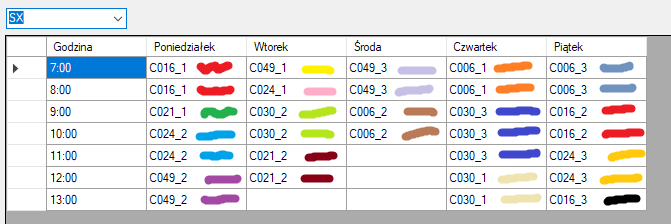
\includegraphics[width=\textwidth] {sx}
	\caption{Najlepszy otrzymany plan zajęć dla najlepszego rozwiązania.}
	\label{fig: sxkopia}
	\end{figure}
	
	\begin{figure}
	\centering
	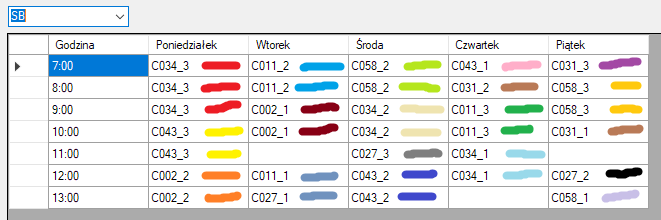
\includegraphics[width=\textwidth] {sb}
	\caption{Najgorszy otrzymany plan zajęć dla najlepszego rozwiązania (2 okienka).}
	\label{fig: sbkopia}
	\end{figure}

Na wykresie przedstawionym na rysunku 6.3 przedstawiono drogę algorytmu jaką musiał pokonać w czasie swojej pracy. Na osi pionowej przedstawiona jest ogólna ocena aktualnego rozwiązania, na osi poziomej przedstawiono liczbę iteracji.

	\begin{figure}
	\centering
	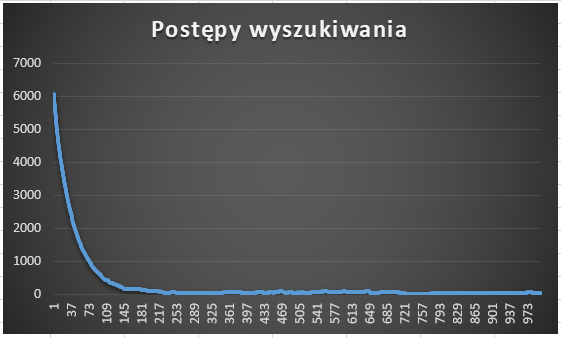
\includegraphics[width=\textwidth] {postepywyszukiwania}
	\caption{Przebieg pracy algorytmu.}
	\label{fig: postepywyszukiwania}
\end{figure}

Najlepszy wynik otrzymany został dla następujących parametrów wejściowych: liczba iteracji - 1000, długość tabu - 500, rozmiar sąsiedztwa  - 300. Liczba iteracji algorytmu została ustalona biorąc pod uwagę czas pracy programu oraz fakt, że liczba ta zazwyczaj wystarczała, by usunąć wszystkie konflikty z planu zajęć. 

Rozmiar sąsiedztwa również w dużej mierze wpływa na czas pracy algorytmu. Z drugiej strony doświadczenia pokazały, że im większe sąsiedztwo tym mniej iteracji potrzebnych do uzyskania lepszych wyników. Rozmiar 300 to około 5\% całego sąsiedztwa możliwego do przeszukania. Ustawienie algorytmu na przeszukiwanie 100 \% sąsiedztwa, spowodowało by wydłużenie pracy algorytmu dwudziestokrotnie. Ustalony rozmiar jest próbą pogodzenia oczekiwań jak najkrótszego czasu pracy algorytmu i jak najlpeszych wyników.

Długość tabu zmienia całkowicie sposób pracy algorytmu. Ustalenie wartości 500 wynikało z obserwacji wyników jakie dostarczał algorytm oraz wykresów, obrazujących jego pracę. Szczegółowe omówienie wpływu parametru długości Tabu przedstawiono w kolejnym podrozdziale.

\section{Znaczenie parametru długości Tabu.}

Algorytm wyszukiwania z Tabu opiera się na algorytmie przeszukiwania lokalnego. Najważniejszą różnicą między tymi algorytmami jest lista Tabu. Dlatego parametr określający długość trwania elementów na liście Tabu ma bardzo duże znaczenie. Zmiana tego parametru powoduje zupełnie inną pracę algorytmu. Potwierdzeniem tego niech będą poniższe wykresy.

Na wykresach zaprezentowanych na rysunkach 6.4 - 6.8 przedstawiono przebieg pracy algorytmu dla parametrów: 1000 iteracji i rozmiarze sąsiedztwa równym 300. Zmieniał się tylko parametr długości Tabu. Jak można zauważyć na rysunku 6.3, algorytm w początkowej fazie pracy znacznie poprawia swój wyniki (z wyniku około 6000 do wyniku 200). Z tego powodu na poniższych wykresach przedstawiono tylko ostatnie 800 iteracji, by obciąć skok i móc zaobserwować zmiany pracy algorytmu w mniejszej skali.

\begin{figure}
	\centering
	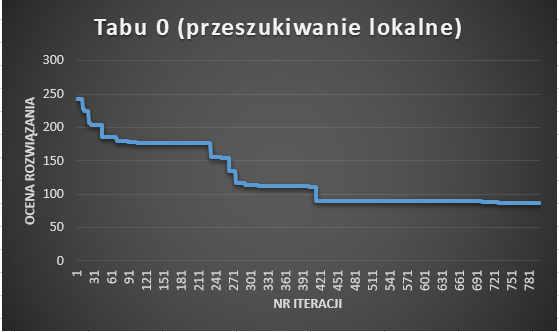
\includegraphics[width=\textwidth] {0}
	\caption{Przebieg pracy algorytmu dla parametru długości Tabu - 0.}
	\label{fig: 0}
\end{figure}

\begin{figure}
	\centering
	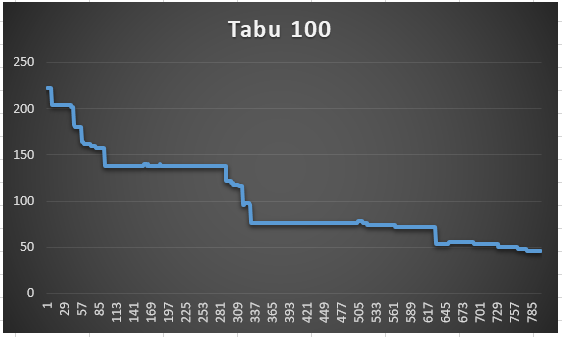
\includegraphics[width=\textwidth] {100}
	\caption{Przebieg pracy algorytmu dla parametru długości Tabu - 100.}
	\label{fig: 100}
\end{figure}

\begin{figure}
	\centering
	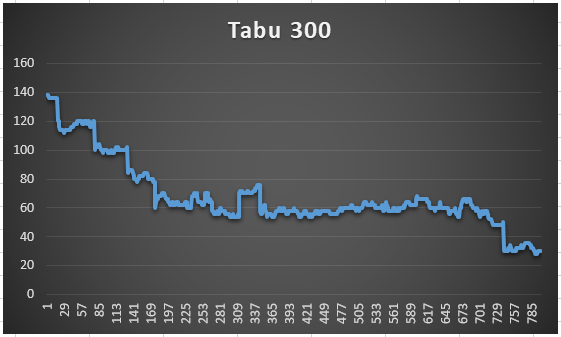
\includegraphics[width=\textwidth] {300}
	\caption{Przebieg pracy algorytmu dla parametru długości Tabu - 300.}
	\label{fig: 300}
\end{figure}

\begin{figure}
	\centering
	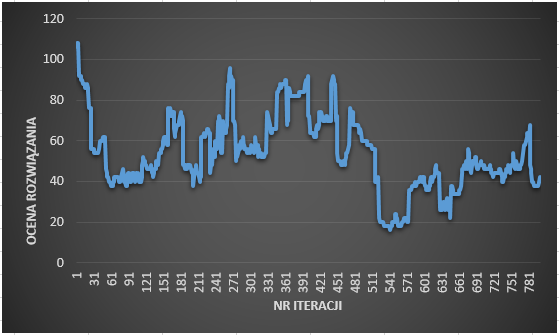
\includegraphics[width=\textwidth] {500}
	\caption{Przebieg pracy algorytmu dla parametru długości Tabu - 500.}
	\label{fig: 500}
\end{figure}

\begin{figure}
	\centering
	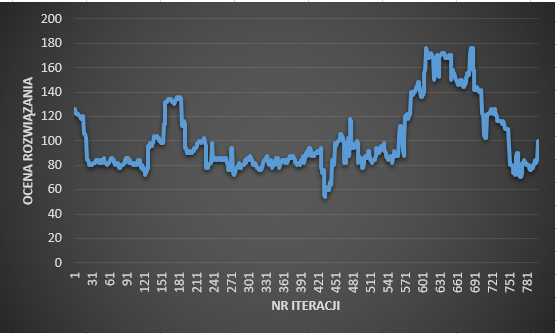
\includegraphics[width=\textwidth] {800}
	\caption{Przebieg pracy algorytmu dla parametru długości Tabu - 800.}
	\label{fig: 800}
\end{figure}

Pierwszy z wykresów (rysunek 6.4) prezentuje pracę algorytmu dla parametru długości Tabu równym 0. Oznacza to, że algorytm w ogóle nie korzysta z listy Tabu. Jest więc to przeszukiwanie lokalne. Jak widać, algorytm przeszukuje tylko wyniki, które mają tą samą ocenę lub wyższą. Na wykresie nie można zauważyć żadnego skoku wartości w górę. Jest to spowodowane wpadaniem algorytmu w lokalne minima, a poprawa rezultatu najczęściej jest skutkiem innego losowego doboru sąsiadów. Wynik jaki udało się osiągnąć to 84.

Drugi wykres (rysunek 6.5) przedstawia przebieg algorytmu dla parametru długości Tabu równego 100. Otrzymany wykres jest bardzo zbliżony do poprzedniego, jednak można zaobserwować małe próby pogorszenia wyników w celu dotarcia do rozwiązania jeszcze lepszego. Najlepszy wynik to 48. Jak widać, 100 ruchów zabronionych z puli 6000 dostępnych (dla tego przypadku testowego), to zdecydowanie za mało, by efektywnie korzystać z zalet wyszukiwania z Tabu.

Na trzecim wykresie (rysunek 6.6) sytuacja wygląda już zdecydowanie lepiej. Długość Tabu równa 300 wymusza na algorytmie przeszukiwanie obszarów, do których dotrzeć można tylko przez pogorszenie bieżącego wyniku. Większe skoki algorytmu to miejsca, w których udało się wyeliminować pewien konflikt zasobów (ocena 20). Mniejsze zmiany obrazują próby minimalizacji okienek (ocena 2 dla jednego okna czasowego). Najlepszy uzyskany wynik to 30.

Czwarty wykres (rysunek 6.7) prezentuje sytuację, w której udało się osiągnąć najlepsze rezultaty (w tym przypadku 18). Najlepszy wynik udało się osiągnąć już w 740 iteracji (540 + 200 iteracji nie przedstawionych na wykresie). Dla parametru długości Tabu równym 500 przeszukiwanie odbywa się już bardzo skokowo. Algorytm nie może wykonać 500 ruchów, które w poprzednich iteracjach najbardziej poprawiły wyniki algorytmu. Dzięki temu jest w stanie dotrzeć do obszarów, które dla przeszukiwania lokalnego są nieosiągalne.

Ostatni wykres (rysunek. 6.8) przedstawia przebieg algorytmu dla parametru długości Tabu równego 800. Przy 1000 iteracjach algorytmu tylko pierwsze 200 ruchów będzie mogło zostać powtórzone. Niestety, tak duża liczba zabronionych ruchów spowodowała, że algorytm zdecydowanie pogorszył swoje wyniki (najlepszy rezultat to 52). Choć program próbował przejść w inne obszary poszukiwań, to nie otrzymano oczekiwanych rezultatów. Najprawdopodobniej, kluczowe ruchy znajdowały się na liście Tabu.